%% LyX 2.1.1 created this file.  For more info, see http://www.lyx.org/.
%% Do not edit unless you really know what you are doing.
\documentclass[12pt,english]{article}
\usepackage[T1]{fontenc}
\usepackage[latin9]{inputenc}
\usepackage[a4paper]{geometry}
\geometry{verbose,tmargin=1.25cm,bmargin=1.25cm,lmargin=1.25cm,rmargin=1.25cm,headheight=1.25cm,headsep=1.25cm,footskip=1.25cm}
\usepackage{graphicx}
\usepackage{babel}
\begin{document}

\title{EM Wave in Drude-material}


\author{Sankeerth.D\\
EE13B102\\
Electrical Engineering}
\maketitle
\begin{abstract}
With a given plasma frequency and collision, various configurations
of EM waves in drude-type material are explored.
\end{abstract}

\section{Introduction}

The convolution is the only extra operation that needs to be performed
when compared to the previous reports. We are convolving an exponential
function (of drude material) with the fields, and then differentiating
this. Instead, first, the exponential is differentiated, and then
convilution is performed. The values to be convolved are stored in
an array.


\section{Observations}

On running the simulation in the case where the top half is filled
with the drude material, the following can be observed. Clearly, since
we can see the spread in the wave width, it can be seen that different
frequencies travel at different speeds in this medium, compared to
the air medium below.

The medium on top is the drude material, and the one on the bottom
is vacuum.

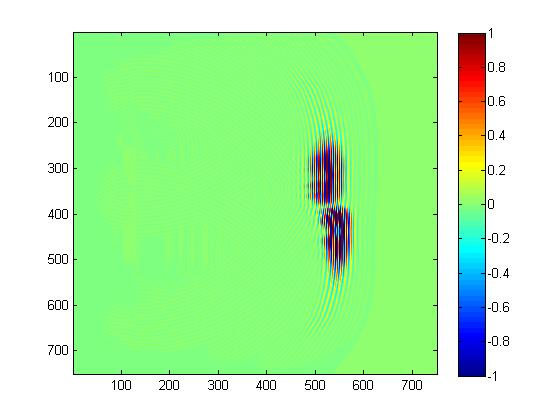
\includegraphics[width=0.45\linewidth]{fig1}

Below the plasma frequency, the wave does not survive in the medium.

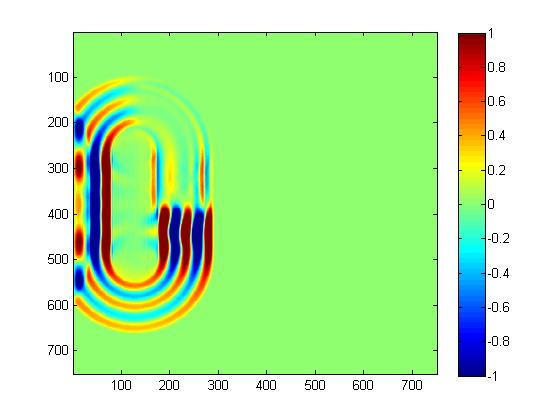
\includegraphics[width=0.45\linewidth]{fig2}


\end{document}
